\documentclass{article}
\usepackage{amsmath}
\usepackage{graphicx} % gráficos
\usepackage[noblocks]{authblk}
%\usepackage{authblk}
%\usepackage[•]{•}ckage{float}
%\usepackage{cite}% para contraer referencias
%\usepackage[usenames]{color}
%\usepackage{showkeys}
%\usepackage{ieeetr}
\usepackage{bm}
\usepackage{hyperref}
\usepackage[normalem]{ulem} %opcional para la correcciones
\newcommand{\abs}[1]{\lvert#1\rvert}
\usepackage{xcolor}
\newif{\ifinclude}
\newcommand{\notaL}[1]{{\color{blue}+L:#1+}}
\newcommand{\notaC}[1]{{\color{green}+C:#1+}}
\newcommand{\notaV}[1]{{\color{red}+V:#1+}}


\title{\textbf{Optimization of Porous Silicon Gradient Refractive
    Index Structures.} }
\author[1]{C. A. Ospina de la Cruz}
\author[2]{W. L. Mochán }
\author[3]{V. Agarwal }

\affil[1]{Posgrado en Ingenier\'ia y Ciencias Aplicadas del Centro de
  Investigación en Ingenier\'ia y Ciencias Aplicadas (CIICAp-IICBA),
  Universidad Autónoma del Estado de Morelos (UAEM), Cuernavaca CP
  62209, México}
\affil[2]{Instituto de Ciencias F\'isica ,Universidad Nacional
  Autonoma de Mexico, Av. Universidad S/N, Col. Chamilpa, 62210
  Cuernavaca, Morelos, Mexico}
\affil[3]{Centro de Investigaci\'on en Ingenier\'ia y Ciencias
  Aplicadas,Universidad del Estado de Morelos, Av. Universidad 1001
  Col. Chamilpa, Cuernavaca, Morelos 62209, Mexico  }
\begin{document}

\maketitle

\begin{abstract}
We propose a simple setup which that the calculation of the current
density as a function of position within an electrochemical cell used
to produce porous Silicon structures with a controlled gradient in their
index of refraction. We produced samples under several conditions and
characterized them with scanning electron microscopy, and
ultraviolet-visible-near infrared reflectance spectroscopy. Our
results allow us to obtain from experiments on a single or just a few
samples a full characterization of the dependence of porosity,
dielectric function and speed of attack on the current density and on
position, so that novel nonhomogeneous devices may be designed and
built.
\notaV{ABSTRACT :  Surfaces with the gradient in the refractive index 
have attracted attention due to their ability to unpair the relation
 between the shape of the optical lens with its optical response. 
  For enhancing the versatility  of electrochemical gradients and its possible usage in
different kinds of devices and applications, it is
desirable to predesign GRIN structures with spatial 
predictability of porosity and the corresponding etching rate.  
In this work, we propose a simple model for the calculation of the current
density as a function of position within an electrochemical cell used
to produce porous silicon structures with a controlled gradient in their
index of refraction. The characterization of some typical PS samples with 
lateral porosity and thickness gradient (produced using pin Pt electrode) 
with scanning electron microscopy and
ultraviolet-visible-near infrared reflectance spectroscopy was 
found to be in conformity with the properties predicted through 
the proposed model. In addition,
as the results allow us to obtain the complete dependence of
porosity, dielectric function and the corresponding etching rate for each 
current density from some measurements performed on a single or 
a couple of samples, the proposed model can facilitate the designing 
of novel sensing devices based on surfaces with lateral gradient in refractive indices.}
Keywords: Porous Silicon; GRIN; Reflectance Spectra.
\end{abstract}
\notaL{Cambié el abstract, pero habrá que revisarlo después.}


\section{Introduction}
\label{sec:introduction}
\notaV{
Introduction 

Surfaces with gradient in the refractive index (GRIN) are of 
importance not only due to the possibility of being able to 
engineer/tune the propagation of light within the structure’s 
surface for applications such as flat lenses, but also for several 
interesting biological applications where the continual topographical 
variation is being exploited \cite{pierscionek2012gradient}. As an example, 
roughness dependent  response of the cells has been tested on such 
materials for applications in medical implants \cite{bai2020bioinspired}.  
 Gradients have also been employed for several 
technological applications such as high-yield screening of catalysts, 
sensing materials and biomolecules \cite{maier2007combinatorial, jayaraman2004construction, 
potyrailo2008combinatorial}
%[W. F. Maier, K. Stçwe, S. Sieg, Angew. 
%Chem. 2007, 119, 6122; Angew. Chem. Int. Ed. 2007, 46, 6016. ;  S. Jayaraman, 
%A. C. Hillier, J. Comb. Chem. 2004, 6, 27; S. Jayaraman, A. C. Hillier, Meas. 
%Sci. Technol. 2005, 16, 5. ; R. A. Potyrailo, V. M. Mirsky, Chem. Rev. 2008, 108, 770.]
%%
Apart from some methods developed by S.E. Fosdick et al \cite{fosdick2010two},
%[JACS  2010, 132, 9226-9227], 
synthesis of  Ag-Au alloy gradients on steel and chemical composition gradients of CdS 
on gold electrode have been made by Shannon’s group\cite{wang2019fabrication}.  
Among the electrochemical methods, compositional and doping density changes 
in the conducting polymer have been used to produce the gradients using Indium tin 
oxide electrode \cite{inagi2010bipolar}
%[S. Inagi, Y. Ishiguro et al Angew Chem Int. Ed. 2010, 49, 10136-10139;
%Angew Chem 2010 122, 10334-10337].   
Electrochemically induced potential gradients have been shown to catalyze the 
reactions and gradient doping of the polymers \cite{qin2020bipolar, ishiguro2011gradient}
%[Gradient Doping of Conducting Polymer 
%Films by Means of Bipolar Electrochemistry Y. Ishiguro, S. Inagi, and T.Fuchigami 
%Langmuir 2011 27 (11), 7158-7162].   (PENDING : few MORE EXAMPLES from last couple of years)
As compared to the above mentioned techniques, a relatively economical, 
fast and easy approach with an additional advantage of being compatible 
with VLSI devices and integrable with microelectronics, for the fabrication 
of refractive index (pore size) gradient has been the development of asymmetric 
electrode configuration in the electrochemical synthesis of porous silicon \cite{sailor2012porous}.  
Although porous silicon initially stimulated the interest of the scientific 
community due to visible PL at room temperature, presently it has 
been accepted as a multifaceted optical material due to its large surface 
area, biocompatibility, ease of fabrication and tunable refractive index. 
Porous silicon emanating applications now cover various fields such as 
chemical and biosensor \cite{kumar2020porous},
%[Porous Silicon Fabry–Pérot Interferometer for
%N-Acetyl-β-d-Glucosaminidase Biomarker Monitoring  D. Nanda Kumar, 
%Nofar Pinker, and Giorgi Shtenberg  ACS Sensors 2020 5 (7), 1969-1976; DOI: 
%10.1021/acssensors.0c00348], 
microelectronics and MEMS \cite{martinez2016dual},as well as a 
range of optical \cite{estevez2014porous} and optoelectronic applications
\cite{ramadan2020fabrication}. Specifically, 
the temporal variation of current density results in the variation of 
porosity along the depth for the easy fabrication of different kinds 
\cite{perez2018reflectivity} of 1D photonics crystals. 
Although the conventional fabrication of PS requires laterally 
homogeneous samples (with same structural characteristics on the 
porous surface), asymmetric configuration to produce porous silicon 
with a lateral gradient (in terms of optical thickness/ pore size and thickness 
of the porous layer) has also been exploited for different applications 
\cite{collins2002determining}. In this configuration, a small platinum electrode (cathode)  
is positioned perpendicular  to the surface of the Si substrate (anode) 
at one end or the center  of the cell, resulting  in a decrease in current 
density  with an increase in the distance from the electrode
 \cite{khung2008using, clements2011mesenchymal}. 
The resulting porous surface can have pore sizes ranging from a few nanometers  
to  few micrometers  \cite{wang2015screening}. The range of the dimensions of the pores and 
the corresponding  thickness obtained on the same chip can be controlled by 
adjusting the location of the pin/circular electrode,  anodizing current density
and etching time period for a given silicon wafer.   Sailor Group 
in 2002 \cite{collins2002determining, sailor2012porous} applied it 
for the determination of protein size. 
Additionally, due to the biocompatible nature of PS, possible gating of 
the optical response by variation in pH of the solution was shown to 
trap/release the biomolecule for possible drug delivery applications. 
 Similar asymmetric electrode configuration was used to fabricate 
 optical filters (multilayered structures) with lateral gradient \cite{li2005painting}
% [Li, Yang Yang, Peter Kim, and Michael J. Sailor. 
% "Painting a rainbow on silicon–a simple method to 
% generate a porous silicon band filter gradient.
% " physica status solidi (a) 202.8 (2005): 1616-1618.] 
for developing ethanol sensor (Sailor 2012)\cite{sailor2012porous}. 
 Additionally it has been shown that the combination of thermal  oxidation  and 
 infiltration of TiO2  by ALD offers the  opportunity to manufacture 
a high refractive indices contrast in visibly transparent GRIN 
optical elements from PS \cite{ocier2017tunable}.    
Kruger et al showed the \cite{krueger2016porous}
%the ...  [ Krueger, Neil A., et al. "Porous silicon gradient 
%refractive index micro-optics." Nano letters 16.12 (2016): 7402-7407.] 
In addition the same group \cite{krueger2018electrochemical}
%[Krueger, Neil A., et al. 
% "Electrochemical Fabrication of Flat, Polymer‐Embedded 
%Porous Silicon 1D Gradient Refractive Index Microlens 
%Arrays." physica status solidi (a) 215.13 (2018): 1800088].  
Recently, J Wang et al. has shown the fabrication of 
miniature spectrometer with PS based rugate filter using 
radial interfacial potential distribution \cite{wang2019fabrication}
%(Wang, Joanna, 
%Michael J. Sailor, and Byoung‐Yong Chang. "Fabrication of a lateral 
%gradient rugate in porous silicon for a miniature spectrometer
%application." ChemElectroChem 6.24 (2019): 5967-5972.
On the other hand, the effect of different topographical
features present on the same chip, has also been 
used to culture / adhesion of certain cells \cite{khung2008using}
In the investigation of such practically applicable systems, 
the spacial predictability of electrochemical gradients can 
be useful for predesigning the devices for different applications.  
In this work, we report a simple analytical model to quantitatively 
analyze the gradient (calculate the porosity /current density and 
thickness) at any point of the GRIN structure.  The paper is organized 
as follows. In Section 2  we report a simple analytical model to calculate 
the current density/porosity and thickness  at any point of the GRIN structure. 
The model contemplates (Dr. Mochan) the formation of electrochemically generated 
porous surface  (applicable/extendible to photonic crystals with lateral gradient) 
with lateral gradient in refractive index  ...with predictable  depth and porosity 
at any point on surface.   In Section 3 we provide experimental details for the 
synthesis of porous silicon samples with lateral refractive index gradient.  
Section 4 includes experimental results and its comparison with numerically 
evaluated parameters. Finally,  the conclusions are given in Section 5
%$ 
%
}

%\notaV{ $Painting a rainbow on silicon - A simple method to  generate a porous silicon 
%band filter gradient. / Li, Yang Yang; Kim, Peter; Sailor, Michael J.
%In: Physica Status Solidi (A) Applications and Materials Science, 
%Vol. 202, No. 8, 06.2005, p. 1616-1618.  (https://doi.org/10.1002/pssa.200461200)
%
%Electrochemical Preparation of Pore Wall Modification Gradients 
%across Thin Porous Silicon Layers
%Corrina M. Thompson, Michel Nieuwoudt, Anne M. Ruminski, 
%Michael J. Sailor, and Gordon M. Miskelly
%Langmuir 2010 26 (10), 7598-7603
%DOI: 10.1021/la904408h
%
% Richardson, Kathleen A., et al. "Advances in infrared gradient 
% refractive index (GRIN) materials: a review." Optical Engineering 59.11 (2020): 112602.
% 
%
%Lavanant, Enora, et al. "Radial gradient refractive index 
%(GRIN) infrared lens based on spatially resolved crystallization 
%of chalcogenide glass." Optical Materials Express 10.4 (2020): 860-867.
%While widely used in the visible, radial gradient refractive 
%index (GRIN) lenses are still elusive in the IR waveband. 
%In this paper we introduce a new method based on spatially
%resolved crystallization of chalcogenide glass to produce such lenses. 
%Optical and structural
%
%Yoon, Sun Mi, et al. "Subwavelength Hollow-Nanopillared Glass 
%with Gradient Refractive Index for Ultralow Diffuse Reflectance 
%and Antifogging." ACS applied materials & interfaces 12.5 (2020): 6234-6242.
%Nanostructured glass with subwavelength hollow nanopillars 
%of diameters of sub-65 nm was fabricated, showing high optical 
%transmittance and ultralow diffuse reflectance. A simple
%process involving single-step plasma etching was used on a 
%glass slide coated with a SiO2...
%
%Perez, Julius C., Tahmid H. Talukdar, and Judson D. Ryckman. 
%"Patterning Refractive Index on the Surface of a Chip by Direct 
%Nanoimprinting." CLEO: QELS_Fundamental Science. Optical Society of America, 2020.
%
%Szymanowski, Hieronim, et al. "Thin SiNC/SiOC Coatings with a 
%Gradient of Refractive Index Deposited from Organosilicon Precursor." Coatings 10.8 (2020): 794.
%  
%Perez, Julius C., Tahmid H. Talukdar, and Judson D. Ryckman.
% "Patterning Refractive Index on the Surface of a Chip by Direct 
% Nanoimprinting." CLEO: QELS_Fundamental Science. Optical Society of America, 2020.
% $
%}




\section{Theory: current density}
\label{sec:theory}
\label{sec:calc-curr-dens}
\notaL{check where acronyms are first defined}
A gradient in the optical properties of porous Silicon (PS) systems may be
obtained by electrochemically attacking a Si surface with a position dependent current
density ${\bm j(\bm r)}$, as the porosity and refractive index depend on
the current density, as well as the etching rate and the thickness of the
porous layer. Nevertheless, it is not a simple task to measure the
{\em local} value of $\bm j(\bm r)$ along the surface. This hampers the
design and optimization of well characterized reproducible GRIN PS
structures.\notaL{Tenemos referencias para afirmar esto?} Thus, we
believe a
system for which the current density field may be
easily computed would be useful.
Though $\bm j(\bm r)$ may be numerically calculated for any
given arbitrary experimental setup,  here we propose a particularly
simple setup that allows an expression for the current in terms
of a series that is rapidly convergent and each of whose terms is a
simple analytic function. With this setup it is easy to characterize
the dependence of different properties of interest on the current, and
this allows the design and optimization of diverse GRIN PS devices.

We assume that our electrolytic cell has the shape of a rectangular
prism (see Fig. \ref{f:celda}) with a horizontal base of sides $a$ and $b$, and
filled with the electrolyte up to a height $c$. We assume that the
walls of the cell are insulating while the bottom is completely
covered with the sample, which is an
electrically grounded relatively good conductor. Within the electrolyte we position an electrode
which we assume is a thin conducting wire, insulated from the electrolyte
but for a small tip, which we approximate as a
point current source.
\begin{figure}
  \centering
  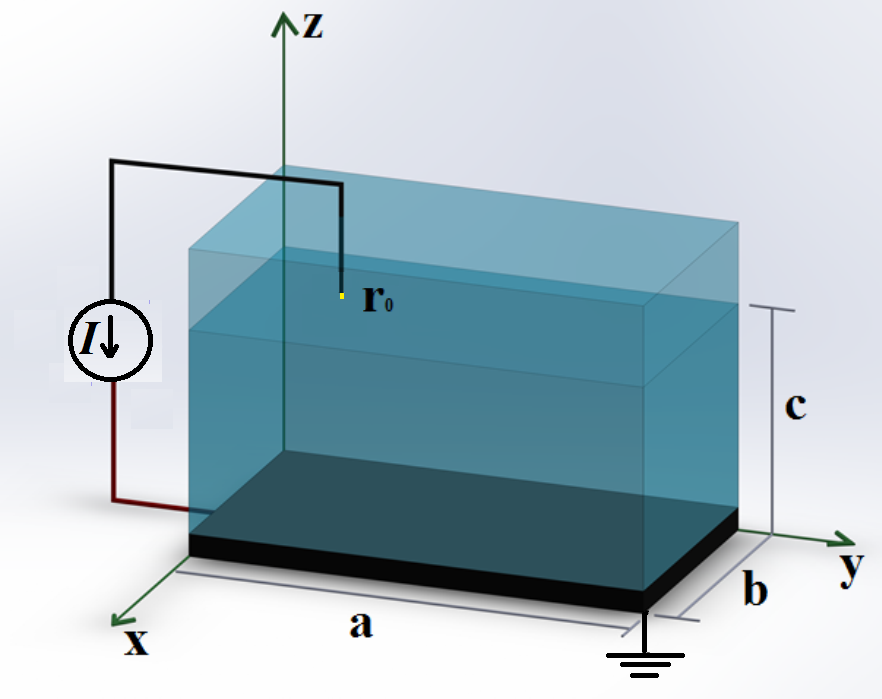
\includegraphics[width=\textwidth]{celdan1.png}
  \caption{Prism shaped electrolytic cell with a rectangular base of
    sides $a$, $b$ filled with electrolyte up to a height $c$. The
    walls of the cell are insulating and the bottom is completely
    covered by the sample, which is assumed to be a good
    conductor. The tip of the electrode is a thin insulated wire
    with just the tip uncovered and located at $\bm r_0=(x_0,y_0,z_0)$ within the
    liquid. The current flows through the electrolyte from the sample
    to the tip.}
  \label{f:celda}
\end{figure}
Within the electrolyte the current density is
\begin{equation}
  \label{eq:j}
  \bm j=\sigma\bm E,
\end{equation}
with
$\sigma$ the conductivity, $\bm E=-\nabla\phi$ the electric field,
and $\phi$ the electric potential. In a
stationary situation
$\nabla\cdot \bm j = \sigma\nabla\cdot\bm E=0$. Thus, the potential
obeys Laplace's equation within the electrolyte,
\begin{equation}
  \label{eq:laplace}
\nabla^{2} \phi=0.
\end{equation}
Consider now an arbitrary closed surface
$\mathcal S$
within the electrolyte that surrounds completely the tip of the
electrode. Integrating $ \bm j$ over this surface we obtain
\begin{equation}
  \label{eq:I}
\int_{\mathcal S'} d\bm a \cdot \bm j = -I,
\end{equation}
where the prime on $\mathcal S'$ means we remove from the surface a
very small hole through which the wire that feeds the current to the
electrode gets
through, and the sign is consistent with the current direction in
Fig. \ref{f:celda}. Assuming the wire is narrower than any other relevant
distance in the system, we may interpret Eq. \eqref{eq:I} as an
integral over a closed surface of the current \eqref{eq:j} within the
electrolyte, ignoring the actual current within the wire. Thus
\begin{equation}
  \label{eq:gauss}
  \int_{\mathcal S} d\bm a \cdot \bm E = -\frac{I}{\sigma}
\end{equation}
Using Gauss's law, we interpret this equation as a source for the
potential in the form of a point charge
\begin{equation}
  q_0 = -\frac{I}{4 \pi \sigma}
\end{equation}
at the position $\bm r_0=(x_0, y_0, z_0)$ of the
tip of the electrode. Note that $q_0$ would be the total charge,
and it shouldn't be further screened through the permittivity of the
electrolyte.

The effective conductivity of the relatively thin sample in contact
with the grounded counter-electrode is large enough that we may assume its
surface $z=0$ is an equipotential.
On the other hand, no current can go across the insulating walls of
the cell, situated at $x=0$, $x=a$,, $y=0$ and $y=b$, nor through the
free surface of the liquid at $z=c$. Thus, the problem to solve is Poisson's
equation with a point charge source
\begin{equation}
  \label{eq:poisson}
  \nabla^2\phi=-4\pi q_0\delta^{(3)}(\bm r-\bm r_0),
\end{equation}
with mixed boundary conditions
\begin{equation}
  \label{eq:ground}
  \phi(x,y,0)=0,
\end{equation}
and
\begin{equation}
  \label{eq:E0}
E_x(0, y ,z)= E_x(a, y ,z)=E_y(x, 0 ,z)=E_y(x, b
,z)=E_z(x, y ,c)=0.
\end{equation}
Here, $\delta^{(D)}$ is Dirac's delta function in $D$ dimensions.
This problem may be solved readily using image charge theory \cite{jackson1999classical}.
The potential within the electrolytic cell coincides
within the region $0\le x\le a$, $0\le y \le b$, $0\le z\le c$
with that an infinite fictitious empty space but for the point charge
$q_0$ at the tip of the electrode at $\bm r_0$, and an array of its fictitious image
charges situated out of the cell. They include an image on the conducting bottom of the
cell, of the opposite charge $-q_0$ and situated at $(x_0, y_0,-z_0)$,
to guarantee that the bottom stays at potential zero.
There are further images on the four walls of the cell, of the same charge $q_0$
and situated at $(-x_0,y_0,z_0)$, $(x_0,-y_0, z_0)$, $(2a-x_0, y_0,
z_0)$ and $(x_0, 2b-y_0,z_0)$ so that, taken one at a time, no current goes across
the corresponding wall. Similarly, there is an image of the same charge $q_0$ at
$(x_0,y_0,2c-z_0)$ so that no current goes across the
surface of the electrolyte. Furthermore, each image charge has to be
further reflected by each of the aforementioned surfaces, yielding
infinitely many new images so that Eqs. \eqref{eq:ground} and
\eqref{eq:E0} hold when all charges are considered together.
\begin{figure}
  \centering
  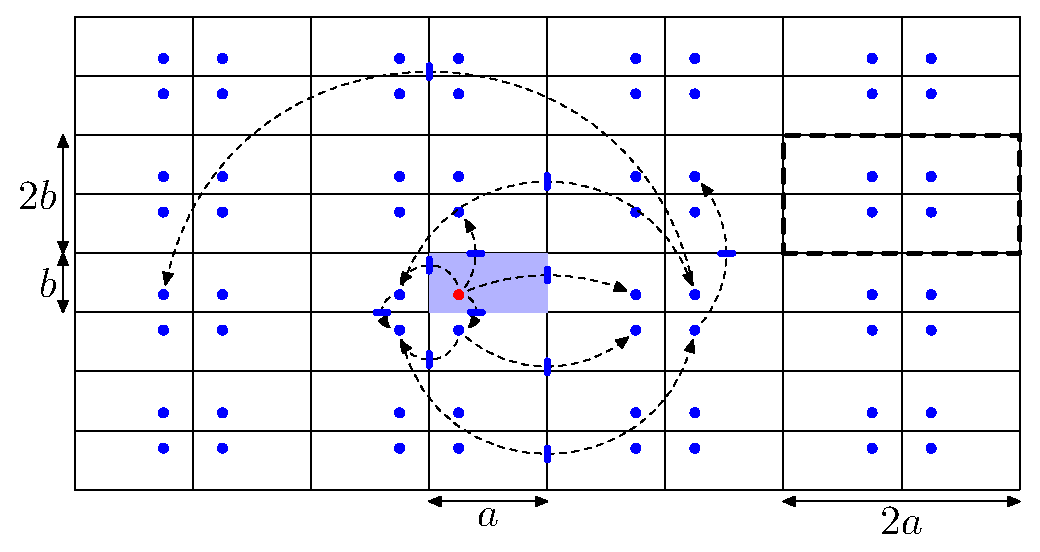
\includegraphics[width=\textwidth]{paper-1}
  \caption{Top view of the $z=z_0$ plane of the fictitious system formed by reflections of
    the electrolytic cell (light blue) showing the charge at the
    tip of the electrode (red dot) and its images on the walls of the
    rectangular cell, the images of its images and so on (blue
    dots). The walls are at $x=0,a$,
    $y=0,b$ (blue lines). The relation of some charges and their images is
    indicated by dashed arrows, with a bar to indicate the
    corresponding reflecting wall. The system may be interpreted as a
    periodic lattice with a rectangular unit cell of size $2a\times 2b$,
    one of which is indicated  by wide dashed lines, and with a basis of four equal
    charges $q_0$ at $(\pm x_0, \pm y_0, z_0)$.}
  \label{fig:topview}
\end{figure}
In Fig. \ref{fig:topview} we illustrate the real charge and all of
its images within the plane $z=z_0$. They form a periodic rectangular
lattice with a unit cell of size $2a\times 2b$ and with a basis of
four equal charges $q_0$ situated at the positions $\bm r_0$, $\bm
r_1=(-x_0, y_0, z_0)$, $\bm r_2=(x_0, -y_0, z_0)$ and $\bm r_3=(-x_0,
-y_0, z_0)$. In Fig. \ref{fig:sideview} we show a lateral view of the
image charges within the plane $y=y_0$.
\begin{figure}
  \centering
  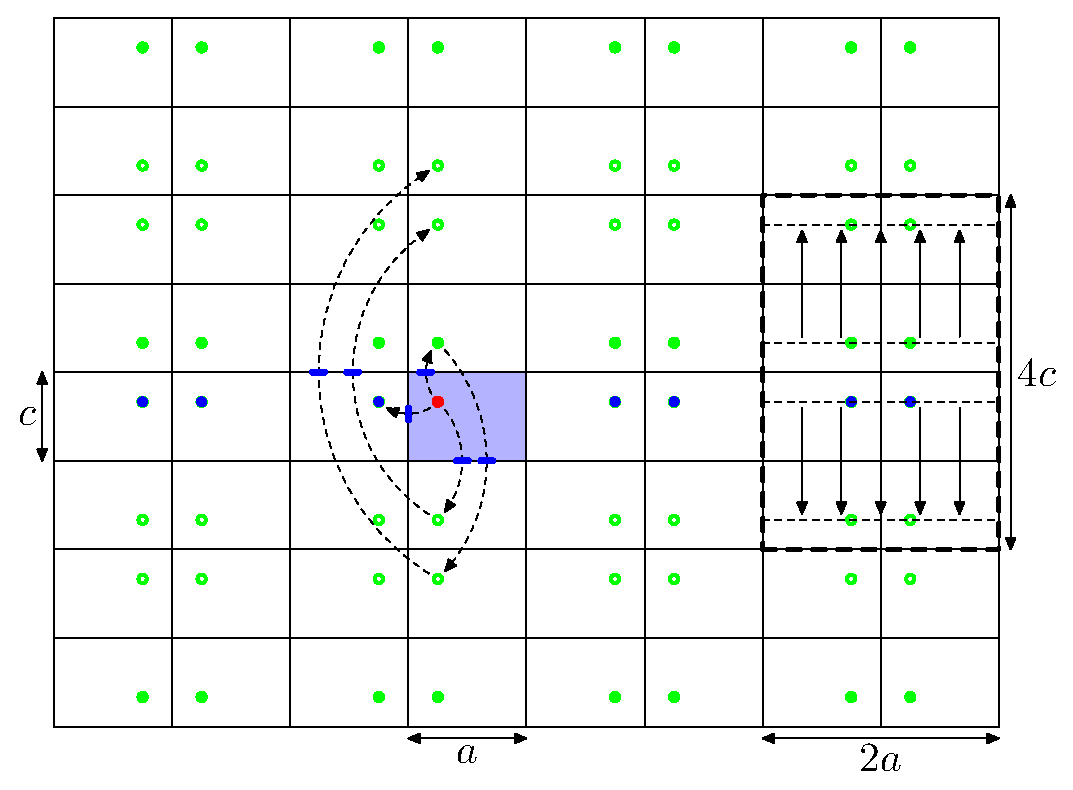
\includegraphics[width=\textwidth]{paper-2}
  \caption{Side view of the $y=y_0$ plane of the fictitious system formed by reflections of
    the electrolytic cell (light blue)
    showing the charge at the tip of the electrode (red dot), its
    images within the plane $z=z_0$ (blue dots), and its images at the
    surface of the sample and the top of the electrolyte (green
    dots). We use solid dots to denote images with the same charge $q_0$
    as that corresponding to the tip of the electrode, and open dots for those of
    opposite charge $-q_0$. The mirror planes that don't invert the charge
    are indicated by blue lines and the mirror plane that inverts the
    charge is indicated by a red line. The relation of some charges and their images is
    indicated by dashed arrows, with a bar to indicate the
    corresponding reflecting wall. The system may be interpreted as a periodic
    lattice with a rectangular unit cell of size $2a\times 4c$, one of
    which is indicated by wide dashed lines, and with a basis of four
    charges $q_0$ and another four charges $-q_0$. Within this cell,
    we indicate its $G=0$ contribution to the electric field (solid
    arrows, see text).}
  \label{fig:sideview}
\end{figure}
Each plane of charges upon reflection on the surface of the sample at
the bottom of the cell yields an
plane of image charges of the opposite sign, while each reflection
on the surface of the liquid yields a plane of charges of the same
sign. The side view may be interpreted as a periodic rectangular
lattice with a unit cell of size $2a\times 4c$ containing a basis of eight point
charges, four positive and four negative. A projection onto the $yz$
plane would similarly yield a rectangular lattice with a  $2b\times4c$
unit cell. Putting everything together, the problem is that of solving
Poisson's equation within an orthothombic lattice of size
$2a\times2b\times4c$ with a basis of 16 point charges of charge $\pm
q_0$ arranged in positive and negative planes.

The electrostatic potential produced by an infinite array of
charges expressed as a sum in real space of Coulomb terms has ill
convergence properties. The potential can be obtained
using the Ewald summation technique \cite{brodka2004ewald}, which yields
two rapidly converging series, one in real space and another one in reciprocal space.
Nevertheless, as we need the potential and the field to obtain the
current density on the surface of the sample on which  no
real nor image charges lie, we may perform a somewhat simpler planewise
summation, where we first obtain the potential and field produced by a
simple periodic lattice of charges using a fast convergent sum over the 2D
reciprocal vectors \cite{kratzer2019basics}, then sum over the charges that form the basis
of the 2D {\em crystal} plane, and finally sum over all the
 planes \notaC{cite{T6,T7}, esta citas las quite porque no puedo contestar esa pregunta de 
 abajo}.\notaL{¿Estas referencias son relevantes? ¿En verdad
 se define en ellas la suma de Ewald por planos? Dime dónde p.f., en qué
 página. Y checa que todas las referencias tengan que ver con lo que decimos}

We consider first a system made of identical {\em unit} charges
ocuppying the positions $\bm R$ of a 2D Bravais lattice $\{\bm R\}$,
which we will take as a rectangular lattice with lattice parameters
$2a$ and $2b$, and lying, for the time being, at the $z=0$ plane.
The potential it produces obeys
\begin{equation}
  \label{eq:poissonRed}
  \nabla^2\phi(\bm r)=-4\pi\sum_{\bm R}\delta^{(2)}(\bm r_\|-\bm
  R)\delta^{(1)}(z)=-\frac{4\pi}{A}\sum_{\bm G}e^{i\bm G\cdot\bm r_\|}\delta^{(1)}(z),
\end{equation}
where $\bm r_\|$ is the projection of the observation position $\bm
r=(x,y,z)$ onto the $xy$ plane, $\{\bm G\}$ is the
reciprocal lattice defined through $e^{i\bm G\cdot\bm R}=1$ for all
$\bm R$ and $\bm G$, $A=4ab$ is the area of the unit cell
and we used the Fourier representation of the 2D
periodically repeated delta function. We introduce a 2D Fourier representation for
the potential
\begin{equation}
  \label{eq:phifourier}
  \phi(\bm r)=\sum_{\bm G}\phi_{\bm G}(z)e^{i\bm G\cdot\bm r_\|}
\end{equation}
where $\phi_{\bm G}(z)$ is the Fourier coefficient of the potential at
the height $z$. Substitution in Eq. \eqref{eq:poissonRed} yields the
ordinary differential equation
 \begin{eqnarray}
 \frac{d^2}{dz^2}\phi_{\bm G}(z)-G^2\phi_G(z)=
   -\frac{4 \pi}{A} \delta^{(1)}(z),
 \end{eqnarray}
for each coefficient, an homogeneous equation for $z\ne0$ which may be trivially
solved. After applying boundary conditions at $z=0$ and regularity
conditions at infinity, we obtain
\begin{equation}
  \label{eq:phiG}
  \phi_{\bm G}(z)=
  \begin{cases}
    -\dfrac{2\pi}{A}\abs{z}&\text{if }G=0,\\
    \dfrac{2 \pi}{AG}  e^{- G \abs{z}}&\text{if }G\neq 0.
  \end{cases}
\end{equation}
The case $G=0$ corresponds to the potential produced by a uniformly charged plane,
while the case $G\ne 0$ is the potential produced by a sinusoidal
charge density on a plane, given by the
symmetric solution that decays exponentially as we get away, upwards
or downwards, from
the source plane. Substituting into Eq. \eqref{eq:phifourier} yields
\begin{eqnarray}
  \label{eq:phiG1}
 \phi(\bm r) = -\frac{2 \pi}{A}  \abs{z} +{\sum_{\bm G}}' \frac{2 \pi
   }{AG} e^{- G \abs{z}} e^{i \bm G\cdot\bm r_\|},
 \end{eqnarray}
where the prime indicates that the term $G=0$ should be ommited from
the sum.

We consider now the basis of our 2D lattice, with equal charges at the
four positions $(\pm x_0, \pm y_0,0)$. Each of the corresponding four
sublattices produces a potential as that in Eq. \eqref{eq:phiG1} but
shifted by the corresponding basis vector, yielding
\begin{equation}
  \label{eq:phiG4}
  \phi(\bm r) = -\frac{8\pi}{A} \abs{z}
    +{\sum_{\bm G}}' \frac{8\pi}{AG} e^{- G \abs{z}}\cos(G_x x_0)
    \cos(G_y y_0) e^{i \bm G\cdot\bm r_\|}.
\end{equation}
Finally, we shift the origin of Eq. \eqref{eq:phiG4} vertically to each of the planes shown in
Fig. \ref{fig:sideview} and multiply by the corresponding charge $q_0$
or $-q_0$ to obtain the contribution to the total potential. The charge $q_0$ corresponds to
the planes with heights of the form $z_0+4nc$ and $-z_0+(4n+2)c$, with
$n=\ldots-2,-1,0,1,2\ldots$ an arbitrary integer, while the charge
$-q_0$ corresponds to the planes with heights $z_0+(4n+2)c$ and
$-z_0+4(n+1)c$.

We concentrate our attention only on the region $0\le z<z_0$ above the
sample but below the electrode. From
Fig. \ref{fig:sideview} we see that the $G=0$
field has contributions only from the charges at $z_0$ and their
images at $-z_0$, and that this contribution is like that of a parallel plate
capacitor $E_{0z}=-4\pi q_0/ab=-16\pi q_0/A$, which corresponds to the
potential $\phi_0=16\pi q_0 z/A$. Other pairs of contiguous planes of with opposite charges
contribute to the field elsewhere. The contributions to the potential
from the $G\ne0$ terms are simple geometric series that may be summed
over $n$ analytically and yield the total potential
\begin{equation}
  \label{eq:phitot}
  \begin{split}
    \phi(\bm r)=&\frac{16\pi q_0}{A}\biggl(z+{\sum_{\bm G}}'\frac{2\sinh
      Gc}{G \sinh 2Gc}\cosh G(c-z_0)\cos G_x x_0 \cos G_y y_0\\
    &\times \sinh Gz\, e^{i\bm G\cdot\bm r_\|}\biggr).
  \end{split}
\end{equation}

Notice that the terms of the sum above converge exponentially to zero
as $G$ increases for any $z$ such that $0\le z <z_0 \le c$, and thus
the sum is convergent. The divergence in the limit $ z
\longrightarrow z_0 $ corresponds to the singularity of the potential
at the position of a point charge, and it is not worrisome, as we are
interested in the field close to bottom $z=0$ of the cell.

The current density normal to the surface may now be obtained as
$j_\perp=-\sigma\partial\phi/\partial z$,
\begin{equation}
  \label{Eq:J}
  \begin{split}
    j_\perp(\bm r) =& \frac{I}{ab}\biggl(1+{\sum_{\bm G}}'\frac{2\sinh
      Gc}{\sinh 2Gc}\cosh G(c-z_0)\cos G_x x_0 \cos G_y y_0\\
    &\times \cosh Gz\, e^{i\bm G\cdot\bm r_\|}\biggr).
  \end{split}
\end{equation}
Eq. \eqref{Eq:J} is a very rapidly convergent expression that allows,
in particular, to calculate the current $j_\perp(x,y,0)$ that attacks
the substrate to produce the PS sample.
Integrating over the surface of the sample we verify
\begin{equation}
  \label{eq:intj}
  \int_0^adx\int_0^bdy\,j_\perp(\bm r)=I,
\end{equation}
as the contributions of opposite non-null reciprocal vectors cancel
out: as expected, all the charges that leave the sample find
their way  to the cathode across the electrolyte.

Using Eq. \eqref{Eq:J} we can correlate the local current density at
the sample as it is prepared with its geometric, structural and optical
properties.

\notaL{Quizás ni merece ser mencionado aquí: For the calculation of the optical properties we use the
well known transfer matrix method \notaL{refs}.}


\section{Procedures}
\label{sec:procedures}
\begin{figure}
  \centering
  \includegraphics[width=.8\textwidth]{paper-3}\\[12pt]
  \includegraphics[width=.8\textwidth]{paper-4}\\[12pt]
  \includegraphics[width=.8\textwidth]{paper-5}

  \caption{Experimental set-up for
    the fabrication of GRIN PS structures. We show a side view of the
    electrochemical cell with the shape of a
    rectangular prism (top panel). We indicate the Si wafer (dark
    gray), the teflon cell (light gray), the sealing o-ring (black
    circles), the insulated feeding cable (white lines within black
    lines), the uncovered platinum tip (white) within the
    electrolyte (blue), the electrical contact below the sample
    (yellow) and the controlled current source. We indicate some geometrical
    parameters of the arrangement $x_0$, $z_0$, $a$ and $c$
    and the current source and a few schematic current flux
    lines. Top and side schematic views of the resulting sample
    (middle and lower panels),
    illustrating eght regions $1\ldots8$ of decreasing porosity,
    illustrating the changes in pore radii,
    length, and density and the porosity gradient.}
  \label{fig:DE1}
\end{figure}

In Fig. \ref{fig:DE1} we show a schematic representation of our
experimental setup to manufacture GRIN PS structures.
As dicussed above, we fabricated an electrolytic cell with the shape of a
rectangular prism on the bottom of which we place a Si wafer which makes
electrical contact to a brass \notaC{ laton. gold plate} 
\notaL{Lo inventé; de qué material es
  el contacto bajo la muestra?} which together make the anode. The
cathode consists of a platinum wire insulated except for a small region
at its tip, which we take as a point current drain.
We also show a schematic drawing of the expected GRIN PS structures,
with a gradient in the porosity, and in the thickness, density and depth
of the resulting pores.

\subsection{Fabrication of GRIN  PS Single Layers}
\label{sec:fabrication-ps-grin}
We manufactured single layer PS structures through electrochemical
anodization of a (100) $p$-type crystalline Si wafer
(resistivity 0.002 - 0.005 $ \Omega\,\text{cm}$), under galvanostatic
conditions. The process was performed at
\notaC{room temperature, no controle latempertaura}
,\notaL{OJO. No controlaste la temperatura} with an
electrolytic mixture of aqueous hydrofluoric
acid (HF) (concentration 48\% wt), glycerol (purity 99.8 \% wt) and
ethanol (purity 99.9\% wt) in a 3:7:1 volume ratio. \notaL{Checa que
  todo esto sí corresponda a tus últimas muestras} \notaC{SI corresponde}
   After the anodizing process, the samples were rinsed with
ethanol (purity: 99.9 $ \% $  wt). The electrolytic cell had the shape
of a rectangular prism as shown in Fig. \ref{fig:DE1}, with a base of
sides $a=2.01\,\text{cm}$ \notaL{Cambié el número, de acuerdo a unas
  mediciones de Cristian} and $b=1.48\,\text{cm}$, with an uncovered sample area
of about $3\,\text{cm}^2$. The height of the liquid was set at
$c=1\,\text{cm}$. The cathode was a
platinum wire that with a diameter of $0.41\,\text{mm}$ insulated by a
teflon cylinder of external diameter $\,2\text{mm}$, with an uncovered
tip located at $\bm r_0=(x_0,
y_0,z_0)=(0.2\,\text{cm},0.74\,\text{cm},0.9\,\text{cm})$. \notaL{Checa todos estos datos}
We manufactured three samples $G_1$, $G_2$ and $G_3$ by applying a
current $I_1=5\,\text{mA}$, $I_2=10\,\text{mA}$ and
$I_3=20\,\text{mA}$, respectively, during a time of $t=250s$.

\subsection{Reflectance Measurement}
\label{sec:refl-meas}
We measured the reflectivity spectra at different positions over our
samples using a {\em Perkin Elmer Lambda 950}
UV-Vis-NIR spectrophotometer.\notaL{Finalmente, ¿fue éste el que se
  usó? Si sí, ¿hay algo internesante que decir sobre el? Cosas como el
tamaño de mancha, resolución espectral, etc.} \notaC{Data collection absoluto
reflectance mode. Spot size, physical setting, width (0.7mm) and length (2.0mm).
Instrument setting, slit width (0.6mm). Method settings 
wavelength from(1400nm) to(300nm)}
 
 For interpretation of the data layer we used
the standard formula \cite{stenzel2015physics} for the reflectance of three media:
air (0) environment, the PS film (1) and the c-Si substrate (2),
 \begin{equation}\label{Eq:ECMR}
   R=\left |\frac{r _ {_ {01}}r _ {_ {12}} e^{2i\psi}}{1+r _ {_
   {01}}r _ {_ {12}} e^{2i\psi}}\right |^2
\end{equation}
where $r_{01}$ and $r_{12}$ are the Fresnel reflectance
coefficients of the air/PS and PS/c-Si interfaces \cite{sattler2017silicon}
and $\psi=k_1^\perp d$, where $k_1^\perp$ is
the component of the wavevector perpendicular to the surface within
the porous layer of thickness $d$. The reflectance depends on the
thickness of the film and on the index of refraction $n_1=n_{\text{PS}}$ of the porous
layer, which we relate to the porosity through Bruggeman's
effective medium theory \cite{theiss1997optical},
\begin{equation}\label{Eq:Brugg}
 p\frac{1-\epsilon_1} {1+\epsilon_1} + (1-p)
  \frac{\epsilon_2 - \epsilon_1}
  {\epsilon_2+\epsilon_1}=0,
\end{equation}
where $\epsilon_2=\epsilon_{\text{Si}}$ is the dielectric function of
the c-Si substrate, and
$\epsilon_1=n_{\text{PS}}^2$ is the dielectric function of the PS layer.
We fitted the reflectance spectra using the porosity $p$ and the
thickness $d$ and a scale calibration factor $s$ as fitting
parameters, and thus, we obtained the porosity
$p$ and the etching rate $v=d/t$ for different values of the local
current density $j_\perp$ expected at several positions on different
samples.

\section{Discussion and Results}
\label{sec:discussion-results}
\subsection{Current Density}
\label{sec:current-density}
\begin{figure}
  \centering
  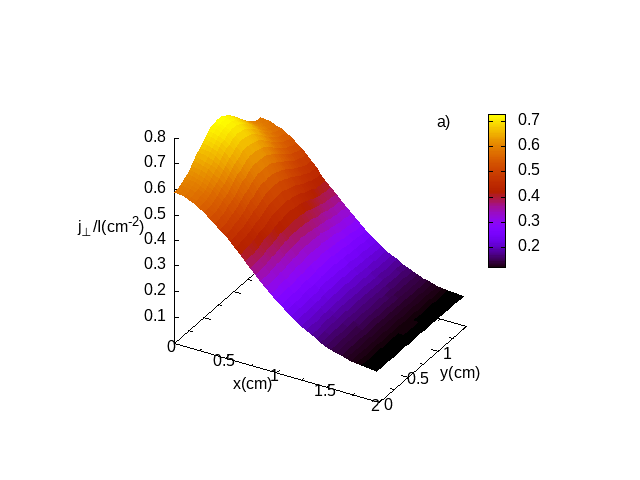
\includegraphics[width=1.2\textwidth]{j_Ivsxy.png}
  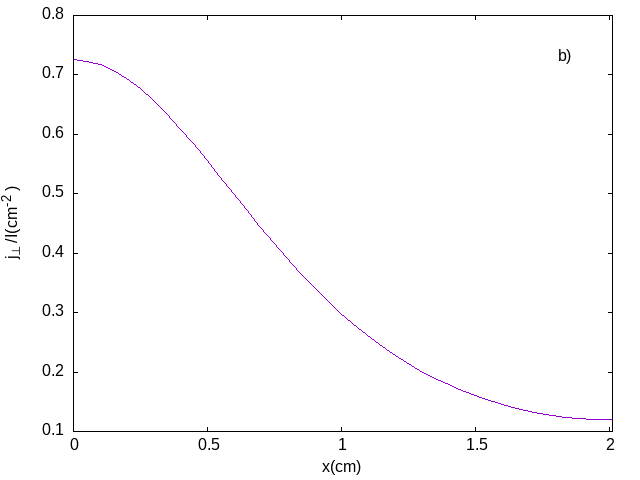
\includegraphics[width=\textwidth]{j_Ivsx.png}
  \caption{Normalized current density $j_\perp(x,y,0)/I$ calculated a
    the surface of the sample through
    Eq. (\ref{Eq:J}) for a
    system as in Figs. \ref{f:celda} and \ref{fig:DE1} for a cell of
    length $a = 2.01\,\text{cm}$ and width $b=1.48\,\text{cm}$, with
    the surface of the electrolyte at a heigth $c=1.0\,\text{cm}$, with a
    point-like electrode at $\bm r_0=(0.2\,\text{cm},
    0.74\,\text{cm},0.9\,\text{cm})$ (top panel). Normalized current
    along the center line $y=0.74\,\text{cm}$ (bottom
    panel).}
  \label{fig:DR1}
\end{figure}
In Fig. \ref{fig:DR1} we show the current density $j_\perp(x,y,0)$ calculated through
Eq. \eqref{Eq:J} at the surface of the sample for our cell, as shown
in Figs. \ref{f:celda} and \ref{fig:DE1} and described in
Sect. \ref{sec:fabrication-ps-grin}). For these parameters we obtained
a large range of values for $ j_\perp/I\sim 0.11-.72\,\text{cm}^{-2}$
that vary mostly along the $x$ direction. Of course, this would differ
for cells with different aspect ratios.

\subsection{Samples }
\label{sec:ps-grin-single}
\begin{figure}
 \centering
  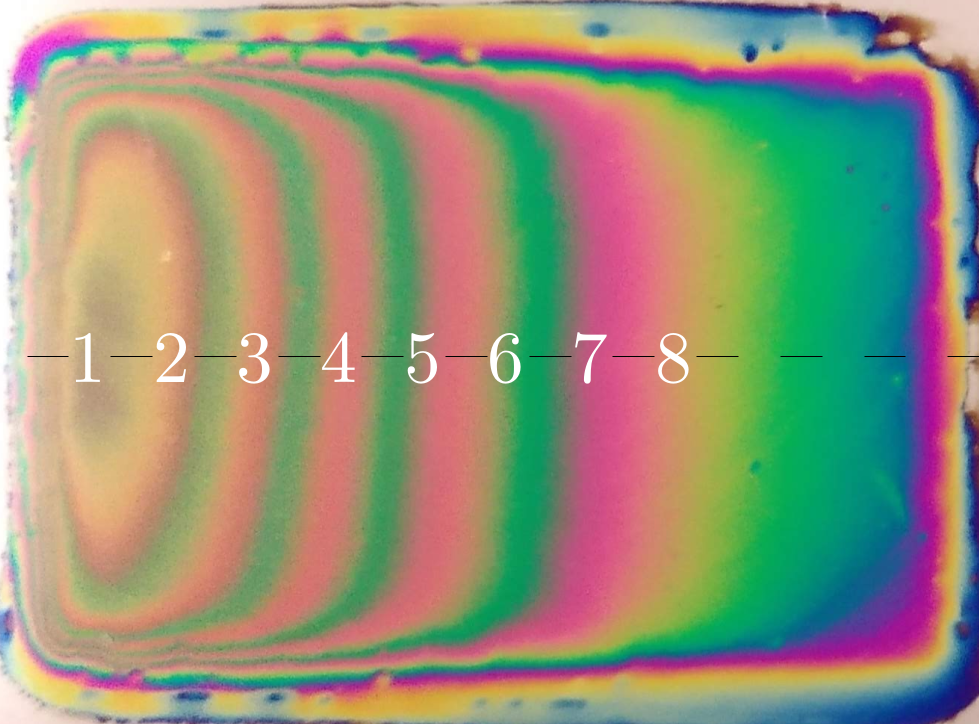
\includegraphics[width=\textwidth]{G3I20proc}
  \caption{ Photograph of sample $G_3$ prepared as described in
    Sec. \ref{sec:fabrication-ps-grin} using the same parameters as
    in Fig. \ref{fig:DR1} with a current $ I_3=20 \text{mA}$,
    during a time $t=250\text{s}$. We indicate eight regions $x_i$
    $(i=1, 2,...8)$ centered at positions,
    $x'_1=0.2\text{cm}$,  $x'_2=0.4\text{cm}$, $x'_3=0.6\text{cm}$,
    $x'_4=0.8\text{cm}$, $x'_5=1\text{cm}$, $x'_6=1.2\text{cm}$,
    $x'_7=1.4\text{cm}$, $x'_8=1.6\text{cm}$, with $y_n=0.74\,\text{cm}$
    on which we measured reflectance spectra. Here,
    $x'_n=x_n+0.14\,\text{cm}$ is the position from the sealing o-ring.}
  \label{fig:SI3}
\end{figure}

In Fig. \ref{fig:SI3} we show a photograph of one of our samples,
$G_3$
prepared as described in Sec. \ref{sec:fabrication-ps-grin}, with the
same conditions as those corresponding to Fig.~\ref{fig:DR1} applying
a current
$I_3=20\,\text{mA}$ during a time $t=250\,s$. We notice a series of
visible interference fringes that get wider as we move towards the
right end of the sample, consistent with a inhomogeneous film that
gets thinner towards the right, and qualitatively consistent with
Fig. \ref{fig:DR1} that shows a current density that decays towards
the right. Equal color lines seem to correspond to iso-current lines of
Fig. \ref{fig:SI3}, except very close to the the walls of the cell,
where the film rapidly becomes very narrow. The reason is that there
is a small region below the cell walls where the electrolyte penetrates
up to the sealing o-ring (see upper panel of
Fig. \ref{fig:DE1}) and towards which the current leaks from the
neighborhood of the wall. The width of this region is
$w=0.14\,\text{cm}$. Thus, we may expect our formula \eqref{Eq:J}
to fail within that region and close to the border, at distances of the order of the radius
of the cross-section of the o-ring, of the order of a milimeter. The
figure shows eight positions
$x'_n=0.2\,\text{cm},0.4\,\text{cm},\ldots,1.6\,\text{cm}$ on which we
measured the near normal incidence reflection spectra of the
sample. Here, we defined $x'_n=x_n+w$ as the distance to the sealing o-ring,
where $x_n$ is the corresponding distance to the wall of the
cell.

From Eq. \eqref{Eq:J} we evaluate the
normalized current density $j_\perp/I$ expected at the positions $n$ indicated in
Fig. \ref{fig:SI3}.
(Table \ref{t:xj}).
\begin{table}
  \centering
  \begin{tabular}{rrr}
    \(x'_n\)(cm) & \(x\)(cm)& \(j_\perp/I\) (\(\text{cm}^{-2})\)\\
    from edge& from wall&\\
    \hline
    0.2 & 0.06 & 0.722\\
    0.4 & 0.26 & 0.672\\
    0.6 & 0.46 & 0.577\\
    0.8 & 0.66 & 0.464\\
    1.0 & 0.86 & 0.360\\
    1.2 & 1.06 & 0.275\\
    1.4 & 1.26 & 0.211\\
    1.6 & 1.46 & 0.167\\
  \end{tabular}
  \caption{Normalized current density $j_\perp/I$ expected at different positions $x'_n$.}
  \label{t:xj}
\end{table}

\subsection{Reflectance}

\begin{figure}
  \centering
  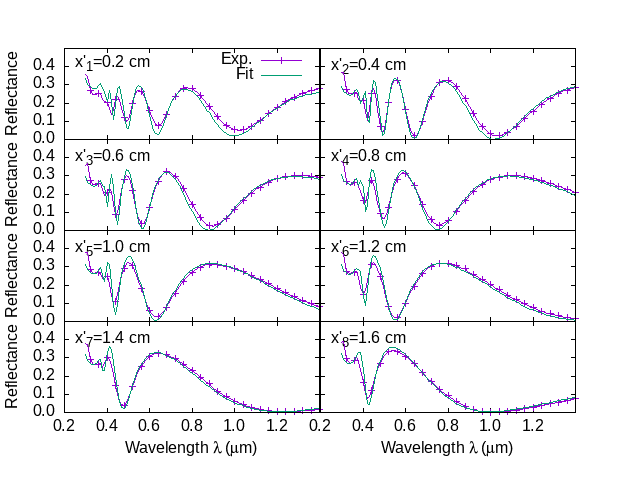
\includegraphics[width=\textwidth]{R5vslambda}
  \caption{Reflectance spectra at different positions
    ($x'_n=0.2-1.6\,\text{cm}$, $y=0.74\,\text{cm}$)
    on sample $G_1$ ($I_1=5\,\text{mA}$). We show
  experimental results and results fitted through
  equations~\eqref{Eq:ECMR} and \eqref{Eq:Brugg}}.
  \label{fig:R5}
\end{figure}
\begin{figure}
  \centering
  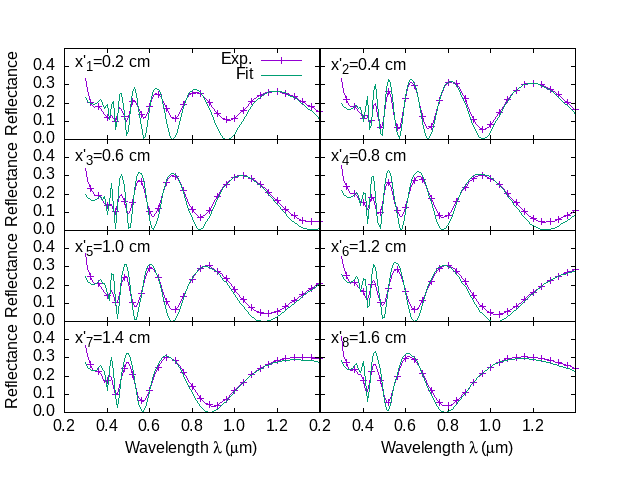
\includegraphics[width=\textwidth]{R10vslambda}
  \caption{Reflectance spectra at different positions
    ($x'_n=0.2-1.6\,\text{cm}$, $y=0.74\,\text{cm}$)
    on sample $G_2$ ($I_1=10\,\text{mA}$). We show
  experimental results and results fitted through
  equations~\eqref{Eq:ECMR} and \eqref{Eq:Brugg}}.
  \label{fig:R10}
\end{figure}

\begin{figure}
  \centering
  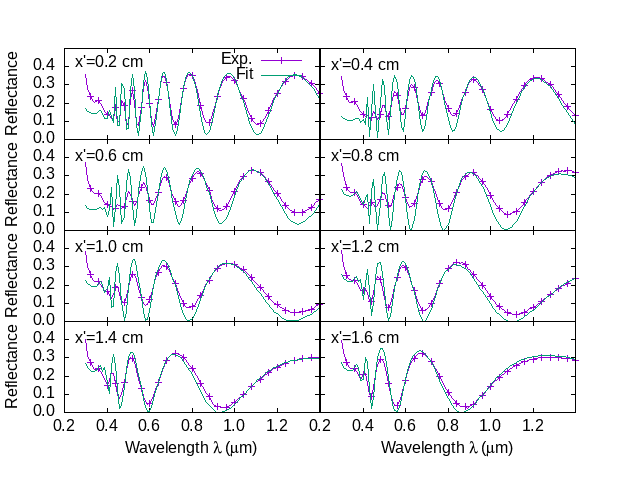
\includegraphics[width=\textwidth]{R20vslambda}
  \caption{Reflectance spectra at different positions
    ($x'_n=0.2-1.6\,\text{cm}$, $y=0.74\,\text{cm}$)
    on sample $G_3$ ($I_3=20\,\text{mA}$) (Fig. \ref{fig:SI3}),
    We show
    experimental results and results fitted through
    equations~\eqref{Eq:ECMR} and \eqref{Eq:Brugg}}.
  \label{fig:R20}
\end{figure}

We measured the reflectance spectra  at the positions indicated in
Fig. \ref{fig:SI3} on our three samples $G_1$, $G_2$,
and $G_3$, prepared using the same procedure
(Sec. \ref{sec:fabrication-ps-grin}) but applying different currents
$I_1=5\,\text{mA}$, $I_2=10\,\text{mA}$, and $I_3=20\,\text{mA}$, . The results are shown in
Figs. \ref{fig:R5}, \ref{fig:R10}, and \ref{fig:R20}.
We fitted the reflectance measurements using Eqs. \eqref{Eq:ECMR} and
\eqref{Eq:Brugg} using the local porosity $p$, and the thickness of the
film  $d$ as
adjustable parameters. We also fitted a scaling parameter $s$ to allow
for calibration variations among spectra. From the thickness we
obtained the etching rate $v=d/t$ at each position. Notice that the fits are reasonably
good. The contrast of the reflectance in the experiment is somewhat smaller
than in our fitted curves. We believe this is due to the finite width
\notaL{beams width=?} \notaC{beams width width (0.7mm) and length (2.0mm)}
of the illuminating beam of our
spectrometer. Thus, as our GRIN sample is not macroscopically homogeneous and its
properties have a gradient, the
experimental results have contributions from regions with slightly
different porosities and thicknesses, averaging out the interference
maxima and minima. We expect microscopic inhomogeneities such as
interface roughness might also reduce the contrast through scattering
and its corresponding apparent dissipation \cite{missoni2020rough}
\notaL{citar a:
  Missoni, Leandro L., Guillermo P. Ortiz, María Luz Martínez Ricci,
  Victor J. Toranzos, and W. Luis Mochán. 2020. “Rough 1D Photonic
  Crystals: A Transfer Matrix Approach.” Optical Materials 109
  (November): 110012. https://doi.org/10.1016/j.optmat.2020.110012.
}.
The loss of contrast is most notable for the thicker regions
towards the left side of Fig. \ref{fig:SI3} and for smaller
wavelengths.

The results obtained from the reflectance fits are summarized in table
\ref{t:jpdv}. Notice that the scaling parameters are close to 1,
showing that the calibration was adequate. \notaL{Is this meaningful?}.

\begin{table}
\centering
\begin{tabular}{lrrrrrr}
  Sample/ & position & density & porosity &
  thickness & scale & rate\\
  $I$ (mA) &$x'_n$ (cm)&  $j$ ($\text{mA}/\text{cm}^2$) & $p$
       & $d$ ($\mu\text{m}$) & $s$ & $v$ (nm/s)\\
\hline
$G_1$/ 5 &0.2 & 3.61 & 0.494 & 0.340 & 0.849&  1.361 \\
         &0.4 & 3.36 & 0.571 & 0.390 & 0.979&  1.558  \\
         &0.6  & 2.88& 0.566 & 0.331 & 0.957&  1.325 \\
         &0.8 & 2.32 & 0.556 & 0.273 & 0.954&  1.093 \\
         &1.0 & 1.80 & 0.559 & 0.227 & 0.995&  0.894 \\
         &1.2 & 1.37 & 0.556 & 0.189 & 0.973&  0.754 \\
         &1.4 & 1.06 & 0.549 & 0.151 & 0.961&  0.605 \\
         &1.6 & 0.83 & 0.552 & 0.124 & 0.990&  0.495 \\
$G_2$/10 &0.2 & 7.22 & 0.591 & 0.635 & 0.856&  2.539 \\
         &0.4 & 6.72 & 0.644 & 0.693 & 0.991&  2.774 \\
         &0.6 & 5.77 & 0.638 & 0.591 & 0.952&  2.363 \\
         &0.8 & 4.64 & 0.626 & 0.533 & 0.980&  2.131 \\
         &1.0 & 3.60 & 0.599 & 0.459 & 0.939&  1.835 \\
         &1.2 & 2.75 & 0.590 & 0.404 & 0.945&  1.618 \\
         &1.4 & 2.11 & 0.575 & 0.338 & 0.936&  1.351 \\
         &1.6 & 1.67 & 0.571 & 0.296 & 0.948&  1.183 \\
$G_3$/20 &0.2 &14.45 & 0.686 & 1.204 & 1.149&  4.818 \\
         &0.4 & 13.44 & 0.713 & 1.193 & 1.078&  4.772 \\
         &0.6 & 11.54 & 0.703 & 1.044 & 1.059&  4.177 \\
         &0.8 &  9.29 & 0.626 & 0.752 & 1.006&  3.006 \\
         &1.0 &  7.20 & 0.625 & 0.538 & 1.010&  2.152  \\
         &1.2 &  5.50 & 0.593 & 0.439 & 0.962&  1.755 \\
         &1.4 &  4.22 & 0.584 & 0.363 & 0.962&  1.453 \\
         &1.6 &  3.33 & 0.591 & 0.339 & 1.011&  1.357 \\
\end{tabular}
\caption{\label{t:jpdv}
  Current density and fitted parameters for saveral positions on
  three samples:  porosity, thickness, scale factor and etching rate.}
\end{table}

From the data in Table \ref{t:jpdv} we can plot the fitted porosity as
a function of the calculated density current, as shown for our three
samples in Fig. \ref{fig:p}.
\begin{figure}
  \centering
  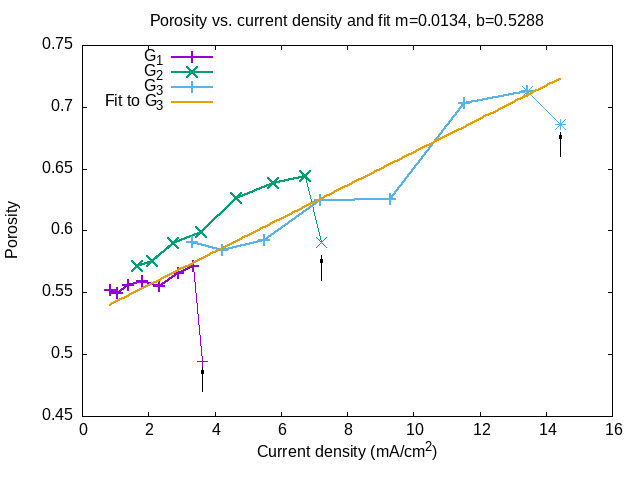
\includegraphics[width=\textwidth]{pvsj}
  \caption{Porosity as a function of current density for three samples
    $G_1$, $G_2$, $G_3$. The data points for each sample are joined by
    thick lines. The arrows point to data that correspond to
    position $x'_1=0.2\,\text{cm}$, joined to the other data by thin
    lines (see text). We include linear fits to the data from
    sample $G_3$ (thick straight line) and to that from all the
    samples (thin straight line). }
  \label{fig:p}
\end{figure}
Notice that for each sample the data points lie around straight lines,
except for one outlier point in each corresponding to position
$x'_1$. As discussed in Sec. \ref{sec:ps-grin-single}, those points
were very close to a wall of the electrolytic cell, so they were
affected by leakage currents towards the underside of the wall.
For this reason, we exclude those points from the following
analysis. We made a linear fit to the data from sample $G_3$ and to
the data from the three samples. A comparison shows that a fit to the
data of just one sample, $G_3$, turns out to be a reasonable predictor for the
porosity of all the samples.  From that fit we obtain that for our
preparation conditions
\begin{equation}\label{eq:p}
  p\approx 0.013\frac{\text{cm}^2}{\text{mA}} j_\perp+0.53.
\end{equation}

Similarly, we can plot the fitted etching rate as
a function of the calculated density current, as shown for our three
samples in Fig. \ref{fig:v}.
\begin{figure}
  \centering
  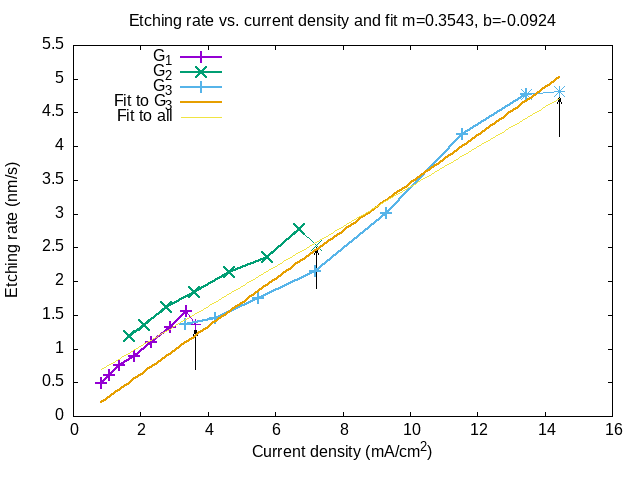
\includegraphics[width=\textwidth]{vvsj}
  \caption{Etching rate as a function of current density for three samples
    $G_1$, $G_2$, $G_3$. The data points for each sample are joined by
    thick lines. The arrows point to data that correspond to
    position $x'_1=0.2\,\text{cm}$, joined to the other data by thin
    lines (see text). We include linear fits to the data from
    sample $G_3$ (thick straight line) and to that from all the
    samples (thin straight line). }
  \label{fig:v}
\end{figure}
As for the porosity, there are outlier points corresponding to the
immediate proximity of the wall of the cell, but the remaining points
lie on straight lines for each sample, and they
may all be approximated by a linear fit to the data of just one
sample, $G_3$, from which we get
\begin{equation}\label{eq:v}
  v\approx 0.35\frac{\text{cm}^2}{\text{mA}}
  \frac{\text{nm}}{\text{s}}j_\perp + 0.092\frac{\text{nm}}{{s}}.
\end{equation}

Using Eqs.  \eqref{Eq:ECMR}-\eqref{eq:v} we can calculate the
reflectance spectra for any
desired current density $j_\perp$ and etching time. This is
illustrated in Fig. \ref{fig:Rvsjl} for the parameters that correspond
to our samples.
\begin{figure}
  \centering
  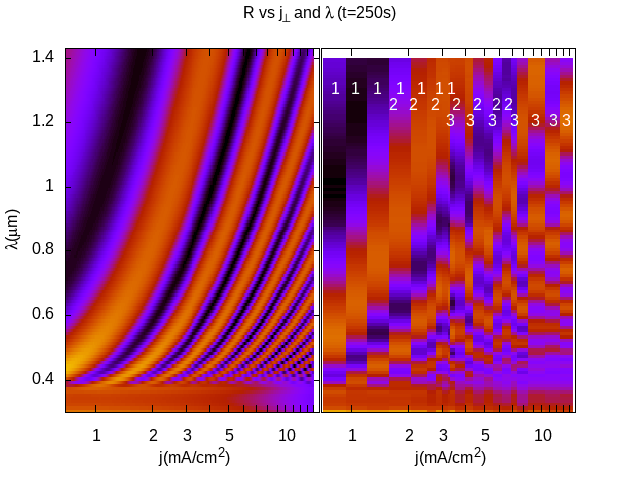
\includegraphics[width=\textwidth]{jlr}
  \caption{Reflection $R$ of a PS film as a function of the current density
    current $j_\perp$ and wavelength $\lambda$ for an etching time
    $t=250\,\text{s}$. Theory (left panel) and experiment (right
    panel, see text). We indicate with the numbers 1, 2, 3 the
    data corresponding to the corresponding samples $G_1$, $G_2$ and
    $G_3$.}
  \label{fig:Rvsjl}
\end{figure}
On the right hand side of the figure we display a quilt made by
patching together the experimental reflectance data corresponding to
Figs. \ref{fig:R5}- \ref{fig:R20}, ordered according to the
corresponding current density as presented in Table
\ref{t:jpdv}. Nevertheless, for the reasons mentioned above, we
eliminated the data corresponding to position $x'_1$ on all
samples. Furthermore, as the results corresponding to sample $G_2$ in
Figs. \ref{fig:p} and  \ref{fig:v} seem shifted with respect to those
of the other samples, in order to facilitate the visualization of the
results, we artificially shifted horizontally towards the
right their contributions to Fig. \ref{fig:Rvsjl} by
$1\,\text{mA}/\text{cm}^2$. Notice that the experimental results may
be grouped along bright and dark bands and that they correspond closely to
those expected theoretically, though the experimental bands are somewhat shifted,
especially for low current densities, and the minima are not as low.

The theoretical reflectance coudl as well be calculated using
\eqref{Eq:ECMR}-\eqref{eq:v} for more complicated structures, in which the
current $I$ is modulated in time, allowing the design and analysis of
non-trivial multilayered GRIN PS structures.


\section{Conclusions}
\label{sec:conclusion}
By choosing a simple geometry for our electrochemical cell, namely, a
rectangular prism, and employing a point-like electrode, we were able
to derive an expression for the calculation of the electric current
density along the surface of a Si sample. The expression was obtained
by using image charge theory and a planewise summation of Coulomb
potentials in 2D reciprocal space, and it is made up of
a rapidly converging sum of analytical terms, just a few of which
should be kept. This allows the characterization
of the porosity of a PS layer and the etching
rate for different values of the etching current density by making
optical measurements on several positions of just a
few samples. We illustrated the procedure with three samples on each of which we
measured reflectance spectra at eight different positions.
Through a optimization procedure we fitted the porosity and etching
rate corresponding to each current density.
We showed that an analysis of the data of just one of the samples, which we chose
as that with the largest current density range, yielded calibration
curves that allow the approximate prediction of the properties of the other
samples. The calibration curves can be used to design and calculate the optical
properties of other systems prepared under similar conditions, such as
multilayered GRIN systems from which photonic crystals, microcavities
and sensors with position dependent properties. This is the subject of
ongoing work. As the etching rate for the formation of porous silicon
and the resulting porosity are very sensitive to the growth conditions
and to the properties of the substrate, such as its doping,
there are no universal calibration curves. Thus, it is useful to have
a procedure that from just one sample can produce calibration curves
that may be employed for other samples grown in the same conditions.

\notaV{By choosing a simple geometry for our electrochemical cell, namely, a
rectangular prism, and employing a point-like electrode, we were able
to derive a simple expression for the calculation of the electric current
density along the surface of a Si sample. The expression was obtained
by using image charge theory and a plane-wise summation of Coulomb
potentials in reciprocal space, and it is made up of
a rapidly converging sum of analytical terms. This allowed us to
characterize the porosity of a PS layer and the etching
rate for different values of the etching current density by making
optical experiments on just a
few samples. We illustrated the procedure with two samples each of which we
measured at three different positions. These calibration curves are
very useful as the etching rate for the formation of porous silicon
and the resulting porosity is very sensitive to the growth conditions
and to the properties of the substrate, such as its doping. Thus,
there are no universal calibration curves. Having obtained these calibration curves
and being able to compute the current density at different positions
allows the prediction of the properties of GRIN structures. We
illustrated this by desigining a PS GRIN microcavity tuned at one
position to a given wavelength. (Q. for Dr. Mochan : Do we intend 
to illustrate the design?) We found a good agreement between its
measured reflectance spectra at different points with the spectra
calculated from the values of the expected local current
density using the calibration curves. We also found good agreement
between the measured and the expected geometry of the system. These
results show that the use of a simple electrolytic cell and our
computational procedure does allow the accurate prediction of the
optical properties of GRIN structures, and thus we believe it will
prove helpful for the design fabrication and characterization of novel}

\section*{Acknowledgments}
\label{sec:acknowledgments}
WLM acknowledges the support of DGAPA-UNAM under grant
IN111119. \notaL{Cristian debe agradecer a conacyt y faltan
  agradecimientos de Vivechna (quizás incluyendo al icf)}
\nocite{*}
\notaL{Manda toda la bibliografía a un archivo .bib}
\notaL{Cuando esté listo, quiero que me expliques por qué incluiste
  cada uno de los artículos citados}
% \bibliography{bibligrin} %Bibliographie
%\printbibliography
%\bibliographystyle{plain}
%\bibliography{bibligrin.bib}
%\medskip
%

\bibliographystyle{unsrt}
%
\bibliography{bibligrin} %Aquí ponen el nombre del archivo .bib




\end{document}
